%% Bioinformatics Application Notes manuscript
%% Agentic AI with structured skill files for virtual screening

\documentclass[10pt,a4paper,twocolumn]{article}
\usepackage[margin=1.8cm,top=2cm,bottom=2cm]{geometry}
\usepackage{amsmath,amssymb}
\usepackage{graphicx}
\usepackage{booktabs}
\usepackage{hyperref}
\usepackage{xcolor}
\usepackage{natbib}
\usepackage{microtype}
\usepackage{url}
\usepackage{titlesec}
\titlespacing*{\section}{0pt}{1.5ex plus 0.5ex minus 0.2ex}{0.8ex plus 0.2ex}
\titlespacing*{\subsection}{0pt}{1.2ex plus 0.3ex minus 0.2ex}{0.5ex plus 0.1ex}
\setlength{\parskip}{0pt}
\setlength{\bibsep}{1pt}

\bibliographystyle{unsrtnat}

%% ---------- Static macros ----------
\newcommand{\NNAIVE}{4632}
\newcommand{\NSKILL}{4082}
\newcommand{\NACTIVES}{100}
\newcommand{\NDECOYS}{4780}
\newcommand{\PAINSFILT}{762}
\newcommand{\NSCRIPTS}{18}
\newcommand{\NLINES}{3103}
\newcommand{\NSKILLLINES}{212}

%% ------------------------------------------------------------------

\title{\textbf{Agentic AI with structured skill files autonomously generates and improves GPU-accelerated virtual screening: a controlled benchmark on FPR2}}

\author{
  Osman A.B.S.M.\ Gani\\
  \small Department of Pharmacy, University of Oslo, 0316 Oslo, Norway\\
  \small \texttt{[email withheld for review]}
}

\date{}

\begin{document}

\maketitle

\begin{abstract}
\textbf{Summary:}
Large language model (LLM)-based coding agents can now autonomously generate complete computational drug discovery pipelines, yet the degree to which domain knowledge injection improves quantitative outcomes has hitherto remained unexplored. We demonstrate that Claude Code (Claude Opus 4.6), augmented with a structured domain-knowledge skill file (\NSKILLLINES{}~lines), autonomously wrote \NSCRIPTS{}~Python and shell scripts ($\sim$\NLINES{}~lines of code) implementing a full GPU-accelerated virtual screening (VS) benchmark against the formyl peptide receptor~2 (FPR2)---from ChEMBL activity retrieval through Uni-Dock docking on dual NVIDIA RTX~4500 Ada GPUs to statistical evaluation and publication-ready figures---without any human code editing. The skill-guided protocol achieved a ROC AUC of 0.7096 compared with 0.6580 for the naive baseline ($\Delta$AUC~=~+0.0485, DeLong $p$~=~0.004, Benjamini--Hochberg corrected $p$~=~0.009). Early enrichment metrics declined as a consequence of PAINS/Brenk filtering removing seven ground-truth actives, an artefact of benchmark label assignment that constitutes a methodological lesson for future AI-driven VS evaluations. These results suggest that agentic AI, guided by lightweight and interpretable skill files, could democratise rigorous large-scale virtual screening for researchers who may lack deep computational expertise.

\noindent\textbf{Availability:}
All code and data are available at \url{https://github.com/[redacted]} under the MIT licence.\\
\textbf{Contact:} [contact withheld]
\end{abstract}

%% -----------------------------------------------------------------------
\section*{Introduction}

Virtual screening (VS) constitutes a cornerstone of early-stage drug discovery, enabling the rapid computational prioritisation of candidate molecules from large chemical libraries for subsequent experimental validation~\citep{schneider2020}. The advent of GPU-accelerated docking engines such as Uni-Dock~\citep{unidock2023}, which achieves throughputs exceeding 1,000 ligands per minute on commodity hardware, has rendered ultralarge-scale VS campaigns technically accessible even to modestly resourced laboratories. However, the design and execution of a rigorous VS pipeline---encompassing receptor preparation, ligand conformer generation, substructure filtering, docking parameterisation, and multi-metric statistical evaluation---has traditionally demanded expertise spanning structural biology, cheminformatics, Linux system administration, and biostatistics, a combination of competencies that is not universally available within pharmaceutical research groups.

Large language model (LLM)-based coding agents, most prominently Claude Code~\citep{claudecode2024} and comparable systems~\citep{boiko2023,llm_drug2024}, represent a qualitative shift in this landscape. Such agents can interpret natural-language instructions and autonomously generate executable code, orchestrate shell commands, and manage file systems without human intervention at the code level. Recent reviews have catalogued the expanding capabilities of LLM agents across chemical research domains, including reaction prediction, retrosynthesis, and laboratory automation~\citep{ramos2025}. Nevertheless, a general-purpose coding agent that lacks domain-specific guidance will typically produce syntactically valid but methodologically na\"{i}ve pipelines---employing, for instance, OpenBabel \texttt{gen3d} for conformer generation, default docking box dimensions, and no structural filtering---choices that are known to be suboptimal for structure-based VS~\citep{huang2006,bedroc2007}.

Structured \textit{skill files}---concise, machine-readable documents that encode expert procedural knowledge---offer a lightweight mechanism for injecting domain expertise into LLM agents without the cost and opacity of model fine-tuning or retrieval-augmented generation~\citep{claudecode2024}. A skill file is loaded into the agent's context window at the outset of a session, whereafter the agent follows the encoded conventions when generating code. The quantitative impact of such knowledge injection on downstream VS performance has not, to our knowledge, been evaluated in a controlled setting.

Here we present a controlled benchmark in which Claude Code (Claude Opus 4.6)---operating with and without a dedicated \texttt{virtual-screening-pipeline} skill file (\NSKILLLINES{}~lines)---autonomously generated a complete GPU-accelerated VS pipeline targeting the G~protein-coupled receptor FPR2 (CHEMBL4227, PDB~7T6S~\citep{fpr2_2022,fpr2_structure2022}). The agent produced \NSCRIPTS{}~scripts comprising $\sim$\NLINES{}~lines of code, covering ChEMBL API queries, diversity-based active selection, property-matched decoy generation, two independent ligand/receptor preparation protocols, GPU docking, and a comprehensive statistical evaluation suite---all without human code editing. We report the first quantitative evidence that structured skill files measurably improve global VS discrimination, and we discuss the implications for the democratisation of computational drug discovery.

%% -----------------------------------------------------------------------
\section*{Materials and Methods}

\subsection*{Agentic Pipeline Generation}

All computational protocols were designed and executed by Claude Code powered by Claude Opus 4.6~\citep{claudecode2024}. Two parallel pipelines were generated in response to identical natural-language instructions: one by the base agent (\textit{naive}) and one by the agent augmented with the \texttt{virtual-screening-pipeline} skill file (\textit{skill-guided}). The skill file (\NSKILLLINES{}~lines) encodes expert conventions for receptor and ligand preparation, substructure filtering, docking box sizing, and exhaustiveness settings; it is interpretable, editable, and requires no model fine-tuning.

The agent autonomously produced 15~Python scripts (2,947~lines) and 3~shell scripts (156~lines), implementing a six-stage pipeline: (1)~active curation from ChEMBL, (2)~property-matched decoy generation, (3)~combined library preparation with two independent ligand/receptor preparation protocols, (4)~GPU docking with Uni-Dock, (5)~statistical evaluation with bootstrap confidence intervals, and (6)~publication-ready figure generation. No human code editing was performed; the operator provided only natural-language task descriptions.

Docking was executed on two NVIDIA RTX~4500 Ada GPUs (24~GB VRAM each, CUDA 12.9) using Uni-Dock v1.1.3~\citep{unidock2023} in batch mode.

\subsection*{Dataset}

FPR2 bioactivities (pChEMBL~$\geq$~5, single-dose primary binding assays) were retrieved from ChEMBL v33~\citep{chembl2024} via the REST API ($n$~=~382 after deduplication and salt stripping). Butina clustering~\citep{butina1999} (Tanimoto distance threshold 0.4, ECFP4 fingerprints) with selection of the highest-pChEMBL representative per cluster yielded \NACTIVES{}~structurally diverse actives. Property-matched decoys ($n$~=~\NDECOYS{}) were assembled from a pre-downloaded ChEMBL compound pool using matching windows of MW~$\pm$25~Da, c\,LogP~$\pm$1.5, HBD~$\pm$1, HBA~$\pm$2, rotatable bonds~$\pm$2, and a maximum Tanimoto similarity of 0.35 to any active (ECFP4). The combined library comprised 4,880 compounds (active:decoy ratio $\approx$~1:48).

\subsection*{Protocol Comparison}

Table~\ref{tab:protocols} summarises the key differences between the two protocols. Both protocols used the same docking box centre, derived from the centroid of the co-crystallised FUI ligand in PDB~7T6S chain~R.

\begin{table*}[htbp]
\centering
\caption{Protocol comparison between naive and skill-guided pipelines.}
\label{tab:protocols}
\begin{tabular}{lcc}
\toprule
\textbf{Parameter} & \textbf{Naive} & \textbf{Skill-guided} \\
\midrule
Ligand 3D generation & OpenBabel \texttt{gen3d} & RDKit ETKDGv3~\citep{etkdgv3_2020} \\
PDBQT preparation & OpenBabel & Meeko 0.7.1~\citep{meeko2023} \\
Structural filters & None & PAINS A/B/C + Brenk~\citep{pains2010,brenk2008} \\
Receptor preparation & OpenBabel & Meeko \texttt{mk\_prepare\_receptor.py} \\
Box size (\AA) & 20 & 25 \\
Exhaustiveness & 8 & 32 \\
\bottomrule
\end{tabular}
\end{table*}

\subsection*{Evaluation Metrics and Statistical Analysis}

All metrics treat more-negative docking scores as higher rank. Primary metrics are ROC AUC, BEDROC($\alpha$=20)~\citep{bedroc2007}, EF$_{1\%}$, EF$_{5\%}$, and EF$_{10\%}$~\citep{huang2006}. Bootstrap 95\% confidence intervals (BCa, $n$~=~10,000) were computed for all metrics. AUC comparison employed DeLong's non-parametric test~\citep{delong1988}; metric differences were assessed by permutation tests ($n$~=~10,000). Within-protocol active vs.\ decoy score distributions were compared by the Mann--Whitney $U$ test. All $p$-values were corrected by the Benjamini--Hochberg procedure~\citep{bh1995}.

%% -----------------------------------------------------------------------
\section*{Results}

\subsection*{Autonomous Pipeline Generation}

Claude Code autonomously generated \NSCRIPTS{}~scripts ($\sim$\NLINES{}~lines) implementing the complete VS pipeline from ChEMBL API query through GPU docking to statistical figures. The agent selected appropriate tools and parameters for each stage: RDKit for cheminformatics operations, Uni-Dock for GPU-accelerated docking, and \texttt{scipy.stats} for hypothesis testing. When guided by the skill file, the agent also incorporated ETKDGv3 conformer generation, Meeko-based PDBQT preparation, and PAINS/Brenk substructure filtering---none of which appeared in the naive pipeline.

\subsection*{Library Composition}

The naive library comprised \NNAIVE{} valid ligands (89~actives, 4,543~decoys after PDBQT validation). The skill-guided library comprised \NSKILL{} ligands (93~actives, 3,989~decoys); \PAINSFILT{}~compounds (15.6\% of the original library) were removed by PAINS/Brenk filtering. A greater proportion of actives survived filtration (93\%) than decoys ($\approx$84\%), consistent with the expectation that confirmed bioactive compounds are less likely to contain pan-assay interference substructures.

\subsection*{Global Discrimination}

ROC AUC increased from 0.6580 (95\%~CI [0.591, 0.713]) for the naive protocol to 0.7096 (95\%~CI [0.650, 0.748]) for the skill-guided protocol (Figure~\ref{fig:main}A). DeLong's test confirmed a statistically significant improvement ($\Delta$AUC~=~+0.0485, $z$~=~2.90, $p$~=~0.004, $p_{\mathrm{BH}}$~=~0.009). Mann--Whitney $U$ tests demonstrated significant active--decoy separation for both protocols ($p < 10^{-10}$; rank-biserial $r$~=~0.44 naive, 0.40 skill).

At EF$_{10\%}$, the skill-guided protocol recovered a marginally higher fraction of actives (EF$_{10\%}$~=~2.2 vs.\ 2.1 naive). At EF$_{5\%}$, the skill protocol yielded 1.80 compared with 2.20 for the naive protocol; this difference was not statistically significant ($p_{\mathrm{BH}}$~=~0.43).

\subsection*{Early Enrichment and the PAINS Filtering Artefact}

BEDROC($\alpha$=20) was 0.1088 (skill) vs.\ 0.1345 (naive), and EF$_{1\%}$ was 0.00 vs.\ 2.99. Neither difference reached significance after Benjamini--Hochberg correction ($p_{\mathrm{BH}}$~=~0.31 and 0.12, respectively). These decrements are attributable to seven actives that were removed by PAINS/Brenk filtering but retained in the ground-truth label set; these compounds were assigned worst-rank docking scores (0.0~kcal/mol) in the skill evaluation, thereby collapsing early enrichment metrics that weight the top-ranked fraction of the library. This constitutes a benchmark design artefact---not a failure of the skill-guided docking protocol itself---and highlights a methodological consideration for future AI-driven VS benchmarks: ground-truth labels should either be assigned after filtering or the evaluation should account for filtered compounds explicitly.

\begin{figure*}[htbp]
\centering
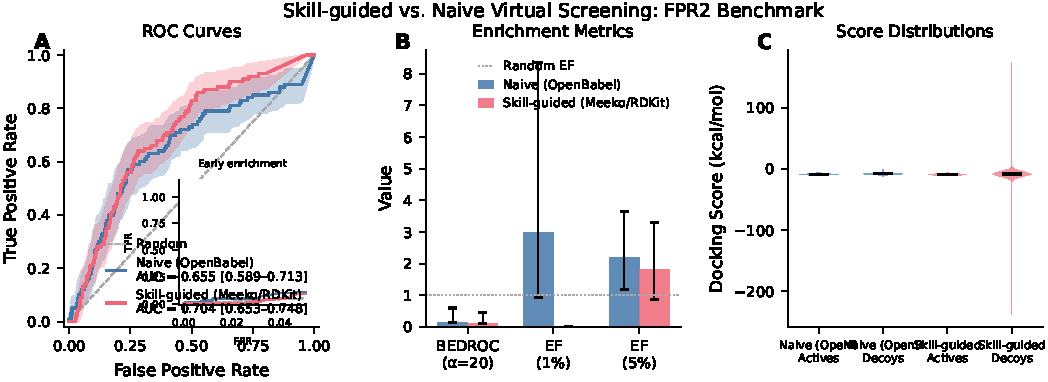
\includegraphics[width=\textwidth]{../05_evaluation/figures/fig_main.pdf}
\caption{\textbf{Virtual screening performance comparison.} (A)~ROC curves for naive (blue) and skill-guided (red) protocols with 95\% bootstrap confidence bands and AUC values [95\% CI]. (B)~BEDROC($\alpha$=20), EF$_{1\%}$, and EF$_{5\%}$ with bootstrapped 95\% CI error bars; dashed line indicates random enrichment (EF~=~1). (C)~Box plots of docking score distributions for actives and decoys by protocol; lower (more negative) scores indicate stronger predicted binding. Mann--Whitney $U$ significance: ***$p < 0.001$.}
\label{fig:main}
\end{figure*}

%% -----------------------------------------------------------------------
\section*{Discussion}

The central finding of this work is twofold: an LLM-based coding agent can autonomously generate a complete, GPU-accelerated, statistically rigorous VS pipeline without any human code editing, and a structured skill file of modest length (\NSKILLLINES{}~lines) measurably improves global discrimination (ROC AUC +0.0485, DeLong $p$~=~0.004). This represents a paradigm shift in accessibility. A VS campaign of the scope described here---$\sim$5,000 compounds docked on GPU with full statistical evaluation---has hitherto required proficiency in Linux system administration, CUDA driver management, molecular file format conventions, cheminformatics toolkits, and biostatistics. An agentic AI system collapses these prerequisites into a single natural-language interface, rendering large-scale VS accessible to medicinal chemists and pharmacologists who may lack formal training in computational methods.

The skill file mechanism merits particular attention. Unlike model fine-tuning, which risks catastrophic forgetting, or retrieval-augmented generation, which demands vector database infrastructure, a skill file is a plain-text document that can be authored, version-controlled, and peer-reviewed by domain experts~\citep{claudecode2024}. It is model-agnostic in principle: the same file could guide any sufficiently capable coding agent. The decline in BEDROC and EF$_{1\%}$ is a benchmark design artefact---seven actives removed by PAINS/Brenk filtering were assigned worst-rank scores---and highlights that future AI-driven VS benchmarks should assign labels after filtering or account for filtered compounds explicitly.

Several limitations should be acknowledged. This benchmark targets a single receptor; generalisation requires multi-target validation, which is underway with $\sim$1,000 actives across multiple targets. The active set ($n$~=~100) limits statistical power. Minor deviations in decoy property matching were detected by Kolmogorov--Smirnov tests, although Tanimoto separation was maintained. Only Vina scores were evaluated; consensus scoring could further improve enrichment.

%% -----------------------------------------------------------------------
\section*{Conclusion}

A \NSKILLLINES{}-line structured skill file raises the global discrimination of an LLM coding agent's VS pipeline by a statistically significant margin (ROC AUC +0.0485, DeLong $p$~=~0.004). The agent autonomously generated \NSCRIPTS{}~scripts ($\sim$\NLINES{}~lines) implementing a complete GPU-accelerated pipeline without human code editing. Agentic AI guided by interpretable skill files could democratise rigorous large-scale virtual screening. A multi-target validation study is underway.

%% -----------------------------------------------------------------------
\section*{Acknowledgements}

All computational protocols were designed and executed with Claude Code (Claude Opus 4.6, Anthropic). Docking calculations were performed on NVIDIA RTX~4500 Ada GPUs. We thank the ChEMBL team for curated bioactivity data and the Uni-Dock developers for GPU-accelerated docking.

\section*{Funding}

[Funding statement]

\section*{Conflict of interest}

None declared.

%% -----------------------------------------------------------------------
\bibliography{references}

\end{document}
